% Build: cd presentation && pdflatex slides.tex && pdflatex slides.tex   (uses ../report/figures/*.pdf)
\documentclass[aspectratio=169,10pt]{beamer}
\usetheme{metropolis}
\usepackage[T1]{fontenc}
\usepackage{booktabs}
\usepackage{tabularx}
\usepackage{tikz}
\usetikzlibrary{arrows.meta,positioning,fit,calc}
\definecolor{cblue}{HTML}{2A78D6}\definecolor{corange}{HTML}{EB6834}\definecolor{caqua}{HTML}{1BAF7A}
\definecolor{ink2}{HTML}{52514E}
\setbeamercolor{frametitle}{bg=black!85}
\setbeamertemplate{frame footer}{Evolving VLM inference for chart QA}
\newcommand{\file}[1]{\texttt{#1}}
\tikzset{box/.style={draw=ink2,rounded corners=2pt,align=center,font=\scriptsize,inner sep=3pt,fill=white},
  arr/.style={-{Stealth[length=4pt]},ink2,thick},
  fname/.style={font=\tiny\ttfamily,text=cblue}}

\title{Evolving Chart-QA Inference for a 2B VLM}
\subtitle{An AlphaEvolve-style system, manual baselines, and an honest holdout}
\author{Ahmadreza Farvardin}
\date{October 2026}

\begin{document}
\maketitle

% ---------------------------------------------------------------- A. Research
\begin{frame}{The problem}
\begin{itemize}
  \item \textbf{Task:} answer CharXiv \emph{descriptive} chart questions (titles, axis labels, tick values, counts,
        legends, layout) with \textbf{Qwen3-VL-2B}, Instruct and Thinking variants.
  \item \textbf{Scoring:} exact match after \texttt{strip()}, case-insensitive: answer \emph{format} matters as much as
        reading the chart.
  \item \textbf{Constraints:} greedy decoding only; only these two models (quantized allowed); speed counts too.
  \item \textbf{Deliverable:} the function \texttt{vlm\_inference(image\_path, question) -> str}, optimized
        (1) by hand and (2) by an AlphaEvolve-style evolution system, for both models.
  \item \textbf{Data:} 1{,}000 labelled validation figures $\times$ 4 questions; the task gives a 128-query dev set.
\end{itemize}
\end{frame}

\begin{frame}{Approach: three tracks, one clean test}
\begin{columns}[T]
\column{0.55\textwidth}
\begin{enumerate}
  \item \textbf{Manual optimization}: one change at a time, measured, committed.
  \item \textbf{Routing}: number-reading / counting questions to Thinking, the rest to Instruct.
  \item \textbf{Evolution}: an LLM rewrites the inference code; fitness on a separate split.
\end{enumerate}
\column{0.43\textwidth}
\small
\begin{tabular}{@{}lrl@{}}
\toprule
split & queries & role \\
\midrule
dev & 128 & manual design \\
evo & 400 & evolution fitness \\
holdout & 800 & \textbf{final test only} \\
reserve & 2{,}672 & single-use checks \\
\bottomrule
\end{tabular}
\end{columns}
\vspace{1em}
Disjoint by figure. All times on one RTX~3090; differences under 10\,\% are noise.
\end{frame}

\begin{frame}{Baseline: the answers were right, the format was not}
\begin{itemize}
  \item Naive Instruct script: \textbf{38.3\,\%} on dev (49/128), 1.95\,s/query; \textbf{25.9\,\%} on holdout.
  \item Main failure: \textbf{verbose answers}. 52 of 128 responses were longer than 60 characters; 3 were correct;
        they took 82\,\% of the time. In 34 of 79 wrong answers the gold answer appears verbatim inside.
  \item \textbf{Step 1, answer extraction} (no prompt change, measured exactly by replaying recorded outputs):
        dev 38.3 $\rightarrow$ 56.2\,\% (\textbf{+17.9}), fresh reserve 32.0 $\rightarrow$ 51.7\,\% (+19.7, 0 broken).
  \item Naive Thinking script: \textbf{0\,\%} on dev: the 128-token limit stops it mid-reasoning.
\end{itemize}
\end{frame}

\begin{frame}{Manual pipeline}
\begin{columns}[T]
\column{0.58\textwidth}
\small
\begin{tabular}{@{}lrrr@{}}
\toprule
Instruct step & dev & reserve & s/query \\
\midrule
baseline & 38.3 & 32.0 & 2.23 \\
1 extraction & 56.2 & 51.7 & 2.23 \\
2a more rules & 57.0 & 51.7 & 2.23 \\
2b answer-only, 64 tokens & 60.2 & 51.2 & \textbf{0.41} \\
2c ``Not Applicable'' check & \textbf{65.6} & \textbf{55.2} & 0.44 \\
\bottomrule
\end{tabular}
\vspace{0.3em}

\footnotesize reserve = reserve[:400]; 2a is a negative result.
\column{0.40\textwidth}
\small
\begin{itemize}
  \item 2b: same accuracy, \textbf{5.4$\times$ faster}.
  \item 2c: abstention recall 20 $\rightarrow$ 44\,\%, precision 100 $\rightarrow$ 73\,\%.
  \item \textbf{Thinking}, step 1: answer after \texttt{</think>}, 1{,}024-token budget, forced answer when it
        runs out: dev 72.7\,\%.
  \item Both manual versions then frozen.
\end{itemize}
\end{columns}
\end{frame}

\begin{frame}{Routing: hypothesis and validation}
\begin{columns}[T]
\column{0.5\textwidth}
\textbf{Hypothesis}
\begin{itemize}\small
  \item Thinking reads numbers better: 24 vs.\ 16 of 51 (reserve[:128]), 32 vs.\ 21 of 49 (dev).
  \item Rule (\file{route\_quant.py}): 7 template phrases $\rightarrow$ Thinking, else Instruct.
  \item Routes all 4{,}000 validation questions as intended (a string-matching check, not generalization).
\end{itemize}
\column{0.48\textwidth}
\textbf{Validation on a fresh slice} (reserve 400--800)
\begin{itemize}\small
  \item Routing \textbf{67.8\,\%} vs.\ Instruct alone 58.8\,\%.
  \item 49 vs.\ 13 discordant answers, McNemar \textbf{$p<0.001$}.
  \item Cost: 28$\times$ slower (10.7 vs.\ 0.38\,s/query).
  \item Became the pre-registered \texttt{best\_accuracy} candidate.
\end{itemize}
\end{columns}
\end{frame}

\begin{frame}{Evolution system design (\file{alphaevolve/})}
\small
\begin{tabularx}{\linewidth}{@{}lX@{}}
\toprule
AlphaEvolve component & this system \\
\midrule
Program database & islands with ring migration; MAP-Elites grid (time $\times$ number-reading accuracy);
parent from top-k (70\,\%) or a random elite \hfill \file{database.py} \\
Prompt sampler & parent code + per-category scores, failures from evo only, inspirations as diffs, sampled
directions, edits already tried \hfill \file{prompt.py} \\
LLM mutation & SEARCH/REPLACE diffs in the EVOLVE block; Gemini 3.1 Flash-Lite (85\,\%) + Gemini 3 Flash (15\,\%)
\hfill \file{llm.py}, \file{diff.py} \\
Evaluation cascade & static checks $\rightarrow$ 8 $\rightarrow$ 64 $\rightarrow$ 400 evo queries (Thinking 4/32/128),
noise-aware promotion \hfill \file{evaluator.py}, \file{checks.py} \\
Loop & synchronous generations; atomic checkpoint; push to \texttt{evo/<run\_id>}; exact resume
\hfill \file{loop.py} \\
\bottomrule
\end{tabularx}
\end{frame}

\begin{frame}{Deviations from AlphaEvolve, and additions}
\begin{columns}[T]
\column{0.48\textwidth}
\textbf{Deviations (and why)}
\begin{itemize}\small
  \item Lockstep generations: one GPU; exact resume.
  \item No meta-prompt evolution: fixed, sampled directions.
  \item Small scale: 72 + 6 children; a full evaluation costs 2.6\,min (Instruct) to $\sim$1\,h (Thinking).
  \item Cascade = growing slices of one benchmark.
  \item Flash-Lite + Flash instead of Flash + Pro.
\end{itemize}
\column{0.5\textwidth}
\textbf{Additions (each after a measured failure)}
\begin{itemize}\small
  \item \textbf{Near-duplicate filter}: reject a child whose edit matches a sibling's (Jaccard $\geq$ 0.8) before GPU.
  \item \textbf{Noise-aware selection}: $<$10\,\% time differences never decide.
  \item \textbf{Static rule checks}: greedy only, allowed model, no gold data.
  \item \textbf{``Already tried'' memory} in the prompt.
  \item \textbf{Pause/resume} on API failure; \texttt{PAUSE} file.
\end{itemize}
\end{columns}
\end{frame}

\begin{frame}{Evolution results}
\begin{columns}[T]
\column{0.5\textwidth}
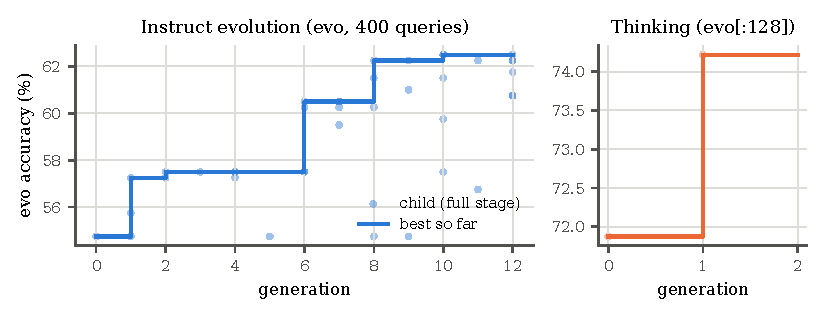
\includegraphics[width=\linewidth]{../report/figures/evolution.pdf}
\column{0.48\textwidth}
\small
\textbf{Instruct} (12 gen.\ $\times$ 6, \$0.23)
\begin{itemize}\small
  \item evo: 54.75 $\rightarrow$ 62.50\,\%; two lineages converge.
  \item \textbf{holdout: 56.0 $\rightarrow$ 62.0\,\% (+6.0, $p=0.0003$)}, from number reading (132 $\rightarrow$ 174 of 326).
\end{itemize}
\textbf{Thinking} (2 gen.\ $\times$ 3, \$0.013)
\begin{itemize}\small
  \item edit: reasoning budget 1{,}024 $\rightarrow$ 512.
  \item \textbf{holdout: $-$33\,\% time} (28.6 $\rightarrow$ 19.3\,s/q), \textbf{+2.2 points} (64.8 $\rightarrow$ 67.0\,\%,
        $p=0.01$).
\end{itemize}
\end{columns}
\end{frame}

\begin{frame}{The routing reversal \quad(headline methodological finding)}
\begin{columns}[T]
\column{0.5\textwidth}
\small
\begin{tabular}{@{}lrr@{}}
\toprule
 & dev & holdout \\
\midrule
Instruct alone (manual) & 65.6 & 56.0 \\
routing (manual models) & \textbf{74.2} & 61.6 \\
Thinking alone (manual) & 72.7 & \textbf{64.8} \\
\bottomrule
\end{tabular}
\vspace{0.5em}

\small Thinking is also better on OCR-type (+19) and layout (+5) questions, which the small design slice had not shown.
\column{0.48\textwidth}
\begin{itemize}\small
  \item Routing was validated against \textbf{Instruct alone}: it won ($p<0.001$).
  \item Against \textbf{Thinking alone} on holdout it loses.
  \item Selection then moved to a \emph{second} fresh slice (reserve 800--1000), not to holdout.
\end{itemize}
\vspace{0.5em}
\alert{A design validated against the wrong baseline can fail on the right one. We caught this only because holdout
had been preserved.}
\end{columns}
\end{frame}

\begin{frame}{Final results on holdout (800 queries)}
\begin{columns}[T]
\column{0.6\textwidth}
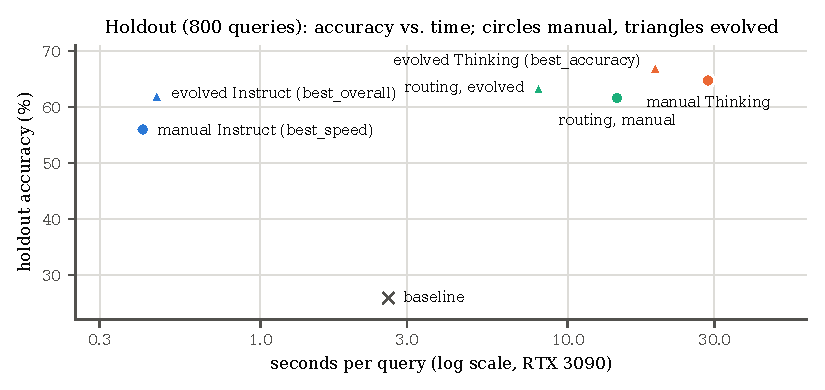
\includegraphics[width=\linewidth]{../report/figures/holdout.pdf}
\column{0.38\textwidth}
\small
\begin{itemize}
  \item \textbf{best\_accuracy}: evolved Thinking, \textbf{67.0\,\%}, 19.3\,s/q (chosen on reserve 800--1000).
  \item \textbf{best\_overall}: evolved Instruct, \textbf{62.0\,\%}, 0.46\,s/q.
  \item \textbf{best\_speed}: manual Instruct, \textbf{56.0\,\%}, 0.41\,s/q (strict rule).
  \item Naive baseline: 25.9\,\%, 2.61\,s/q.
\end{itemize}
\end{columns}
\end{frame}

\begin{frame}{Overfitting audit}
\small
\begin{tabularx}{\linewidth}{@{}llX@{}}
\toprule
split & used for & its numbers are \\
\midrule
dev & manual rules, prompts, token limit & fitted (dev$-$reserve gap grew 4.5 $\rightarrow$ 10.4 points) \\
reserve[:400] & keep/drop decisions & partly tuned \\
reserve[400:800] & routing validation (once) & honest single use \\
reserve[800:1000] & best\_accuracy / best\_speed selection (once) & honest single use \\
evo & evolution fitness & training numbers \\
holdout & final comparison only & \textbf{the primary evidence} \\
\bottomrule
\end{tabularx}
\vspace{0.8em}
\begin{itemize}\small
  \item Holdout informed one decision (\texttt{best\_overall}), where the margin makes the bias negligible.
  \item The routing phrases come from CharXiv's template source code, not from its answers.
\end{itemize}
\end{frame}

% ---------------------------------------------------------------- B. Implementation and workflow
\begin{frame}{Repository: which file does what}
\scriptsize
\begin{tabularx}{\linewidth}{@{}p{0.36\linewidth}X@{}}
\toprule
README deliverable / file & what it is \\
\midrule
\file{manual\_instruct.py}, \file{manual\_thinking.py} & hand-optimized pipelines (frozen at step 2c / step 1) \\
\file{evolve\_instruct.py}, \file{evolve\_thinking.py} & the evolution systems: run configuration + CLI over \file{alphaevolve/} \\
\file{evolved\_instruct.py}, \file{evolved\_thinking.py} & best evolved programs (\texttt{g010\_c01}, \texttt{g001\_c00}) \\
\file{best\_accuracy.py} & = evolved Thinking (selected on reserve 800--1000) \\
\file{best\_speed.py} & = manual Instruct \\
\file{best\_overall.py} & = evolved Instruct \\
\file{evaluate.py} & evaluator: original scoring + CLI, splits, detailed scores JSON \\
\file{starting\_scripts.py}, \file{route\_quant.py} & naive baseline; routing rule (manual design) \\
\file{reproduce.sh} & one command: setup check, tests, all programs on dev (\texttt{--holdout}, \texttt{--evolve}) \\
\file{alphaevolve/} & database, prompt, llm, diff, checks, evaluator, loop, cli \\
\file{scripts/} & replay, candidate runner, figures, zip builder, LLM check, queue scripts \\
\file{scores/}, \file{population/}, \file{analysis/} & every evaluation, every evolution run, probe data \\
\file{report/}, \file{RESULTS.md}, \file{CONTRACT.md} & the paper; the results log; controller/runner contract \\
\bottomrule
\end{tabularx}
\end{frame}

\begin{frame}{How the evolution loop works}
\centering
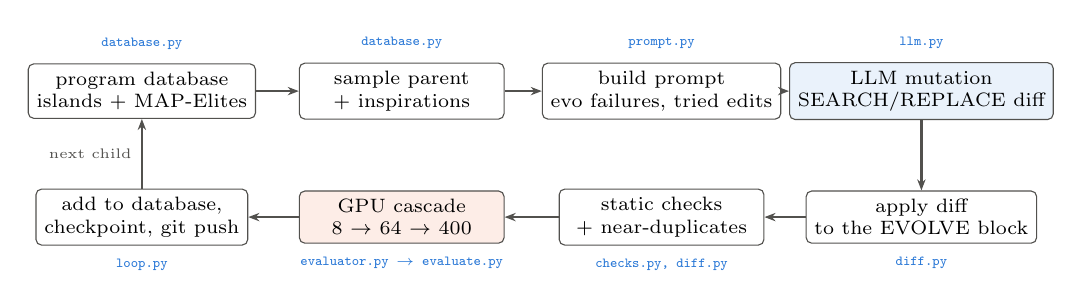
\begin{tikzpicture}[x=3.3cm,y=1.6cm]
  \node[box,minimum width=2.6cm] (db) at (0,0) {program database\\islands + MAP-Elites};
  \node[box,minimum width=2.6cm] (samp) at (1,0) {sample parent\\+ inspirations};
  \node[box,minimum width=2.6cm] (prompt) at (2,0) {build prompt\\evo failures, tried edits};
  \node[box,minimum width=2.6cm,fill=cblue!10] (llm) at (3,0) {LLM mutation\\SEARCH/REPLACE diff};
  \node[box,minimum width=2.6cm] (diff) at (3,-1) {apply diff\\to the EVOLVE block};
  \node[box,minimum width=2.6cm] (checks) at (2,-1) {static checks\\+ near-duplicates};
  \node[box,minimum width=2.6cm,fill=corange!12] (casc) at (1,-1) {GPU cascade\\8 $\rightarrow$ 64 $\rightarrow$ 400};
  \node[box,minimum width=2.6cm] (ckpt) at (0,-1) {add to database,\\checkpoint, git push};
  \draw[arr] (db) -- (samp); \draw[arr] (samp) -- (prompt); \draw[arr] (prompt) -- (llm);
  \draw[arr] (llm) -- (diff); \draw[arr] (diff) -- (checks); \draw[arr] (checks) -- (casc);
  \draw[arr] (casc) -- (ckpt); \draw[arr] (ckpt) -- node[left,font=\tiny]{next child} (db);
  \node[fname,above=0.5mm of db] {database.py}; \node[fname,above=0.5mm of samp] {database.py};
  \node[fname,above=0.5mm of prompt] {prompt.py}; \node[fname,above=0.5mm of llm] {llm.py};
  \node[fname,below=0.5mm of diff] {diff.py}; \node[fname,below=0.5mm of checks] {checks.py, diff.py};
  \node[fname,below=0.5mm of casc] {evaluator.py $\rightarrow$ evaluate.py}; \node[fname,below=0.5mm of ckpt] {loop.py};
\end{tikzpicture}
\vspace{0.8em}

\small Rejected children (duplicates, invalid edits, rule violations) never reach the GPU. A child passes the 64-query
check if it is within a margin of its parent or clearly faster; only full-stage children enter the grid.
\end{frame}

\begin{frame}{Infrastructure and operations}
\begin{columns}[T]
\column{0.5\textwidth}
\begin{itemize}\small
  \item \textbf{Hardware}: rented RTX 3090 (24\,GB), VS Code Remote-SSH; earlier baseline on a Colab T4.
  \item \textbf{Mutation LLM}: Gemini via ArvanCloud's OpenAI-compatible gateway
        (\texttt{\footnotesize api.arvancloudai.ir/v1}): Gemini's API is not available where the machine is hosted.
        Cost \$0.24 for both reported runs.
  \item \textbf{Git}: repo-only deploy key on the GPU; one branch per evolution run.
\end{itemize}
\column{0.48\textwidth}
\begin{itemize}\small
  \item \textbf{Autonomous runs}: chained tmux queues (evolution $\rightarrow$ holdout jobs), each job committing its
        own scores.
  \item \textbf{Robustness}: checkpoint per generation, resume from cache, retry vs.\ pause on API errors,
        \texttt{PAUSE} file, push timeout.
  \item \textbf{Claude Code}: AI coding assistant for code, experiment runs and documentation; the author made
        and reviewed the decisions.
\end{itemize}
\end{columns}
\end{frame}

\begin{frame}{End-to-end workflow}
\centering
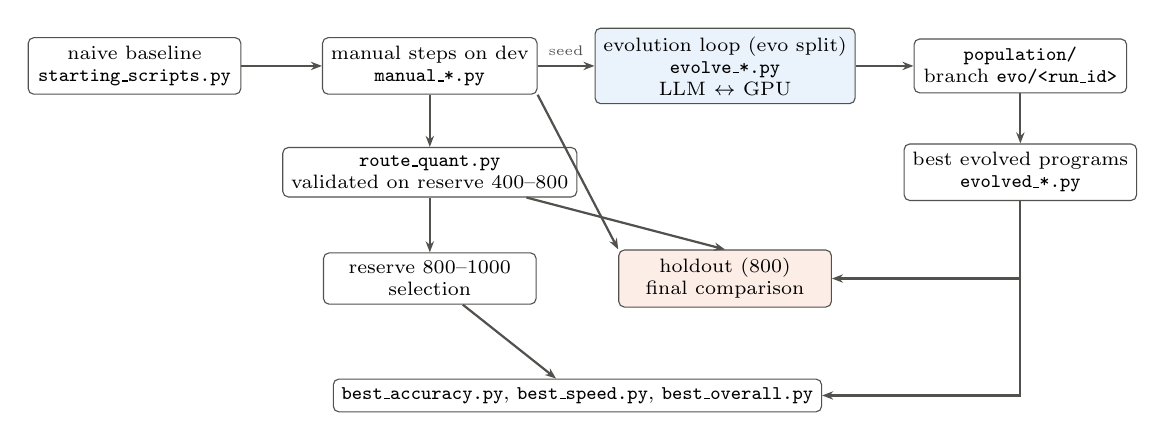
\begin{tikzpicture}[x=3.75cm,y=1.35cm]
  \node[box,minimum width=2.7cm] (base) at (0,0) {naive baseline\\\file{starting\_scripts.py}};
  \node[box,minimum width=2.7cm] (man) at (1,0) {manual steps on dev\\\file{manual\_*.py}};
  \node[box,minimum width=2.7cm,fill=cblue!10] (evo) at (2,0) {evolution loop (evo split)\\\file{evolve\_*.py}\\LLM $\leftrightarrow$ GPU};
  \node[box,minimum width=2.7cm] (pop) at (3,0) {\file{population/}\\branch \texttt{evo/<run\_id>}};
  \node[box,minimum width=2.7cm] (route) at (1,-1) {\file{route\_quant.py}\\validated on reserve 400--800};
  \node[box,minimum width=2.7cm] (bestev) at (3,-1) {best evolved programs\\\file{evolved\_*.py}};
  \node[box,minimum width=2.7cm,fill=corange!12] (hold) at (2,-2) {holdout (800)\\final comparison};
  \node[box,minimum width=2.7cm] (sel) at (1,-2) {reserve 800--1000\\selection};
  \node[box,minimum width=6cm] (best) at (1.5,-3.1) {\file{best\_accuracy.py}, \file{best\_speed.py}, \file{best\_overall.py}};
  \draw[arr] (base) -- (man); \draw[arr] (man) -- node[above,font=\tiny]{seed} (evo); \draw[arr] (evo) -- (pop);
  \draw[arr] (pop) -- (bestev); \draw[arr] (man) -- (route);
  \draw[arr] (bestev) |- (hold); \draw[arr] (man.south east) -- (hold.north west); \draw[arr] (route) -- (hold.north);
  \draw[arr] (route) -- (sel); \draw[arr] (bestev.south) |- (best.east); \draw[arr] (sel) -- (best);
\end{tikzpicture}
\vspace{0.3em}

\small\file{reproduce.sh} re-runs the evaluation side; \file{scores/} holds every number shown.
\end{frame}

\begin{frame}{Lessons and limitations}
\begin{itemize}\small
  \item \textbf{Evolution prefers easy mutations}: it halved the Thinking budget; a measured intervention (stop before the
        4th ``Wait'') cut $\sim$60\,\% of reasoning tokens with accuracy kept or raised, and was suggested first.
  \item \textbf{Diversity failure}: 4 of 6 Thinking children were byte-identical despite the ``already tried'' list.
  \item \textbf{Cascade}: net 10\,\% GPU saving on Instruct (filters $+$28\,min, early stops $+$24, small-stage overhead
        $-$36): cheap full evaluations and a 75\,\% pass rate make it break even; it pays off for Thinking.
  \item \textbf{Negative result}: more extraction rules did not help (dev +1, reserve +0).
  \item \textbf{Method}: validate against the strongest baseline, and keep one split untouched.
  \item \textbf{Limits}: small runs (72 + 6 children); one GPU; speed work (fast processor, compiled decoding, vLLM)
        deferred.
\end{itemize}
\end{frame}

\begin{frame}[standout]
Questions?

\vspace{1em}
{\normalsize
Repository (private): \texttt{github.com/ahmadrezafarvardin/evolving-vlm-inference}\\[0.5em]
\texttt{bash reproduce.sh} \quad (dev, $\sim$2--3\,h)\\
\texttt{bash reproduce.sh --holdout} \quad (+$\sim$14\,h)\\
\texttt{python evolve\_instruct.py} \quad (needs \texttt{ARVAN\_API\_KEY})}
\end{frame}

\end{document}
